\documentclass[10pt,journal]{IEEEtran}
\usepackage[spanish]{babel}
\usepackage[T1]{fontenc}
\usepackage{amsmath}
\usepackage{float}
\usepackage{graphicx}
\usepackage{booktabs}
\usepackage[pdfauthor={Jheison Martinez Bolivar},pdftitle={Prediccion de la Excentricidad Orbital de Exoplanetas mediante Aprendizaje Supervisado},colorlinks,linkcolor=blue,citecolor=green,urlcolor=cyan]{hyperref}

\begin{document}

  \title{Predicci\'on de la Excentricidad Orbital de Exoplanetas mediante Aprendizaje Supervisado:\\
    Regresi\'on Lineal vs. Random Forest}

  \author{
    Jheison Martinez Bolivar\\
    \textit{Maestr\'ia en Inteligencia Artificial}\\
    \textit{Universidad de La Salle, Bogot\'a, Colombia}\\
    \IEEEmembership{jhmartinez07@unisalle.edu.co}
  }
  \maketitle
  \markboth{Universidad de La Salle --- Aprendizaje de M\'aquina. Agosto 2026}{}

  \begin{abstract}
    Este trabajo aplica dos modelos de aprendizaje supervisado ---regresi\'on lineal y Random Forest--- para predecir la excentricidad orbital (\texttt{orbital\_eccentricity}) de exoplanetas a partir del conjunto de datos NASA Exoplanet Archive Intelligence (6\,150 registros). Tras analizar la distribuci\'on de valores nulos en el Exploratorio de Datos (EDA), se justific\'o la excentricidad como variable objetivo dada su presencia de 15.25\,\% de datos faltantes y su alto valor astrof\'isico. Con un preprocesamiento de limpieza y escalado estandarizado (\texttt{StandardScaler}), se particionaron los datos (80\,\% entrenamiento, 20\,\% prueba). La regresi\'on lineal obtuvo $R^2 = 0.2721$ ($RMSE = 0.1158$, $MAE = 0.0681$), mientras que Random Forest ($n\_estimators=100$) alcanz\'o $R^2 = 0.3850$ ($RMSE = 0.1065$, $MAE = 0.0578$). Los resultados demuestran que las relaciones din\'amicas entre las propiedades planetarias y estelares son esencialmente no lineales y que los m\'etodos de ensamble capturan de manera superior estas interacciones complejas. El cuaderno con la implementaci\'on completa se encuentra disponible en Google Colab: \url{https://colab.research.google.com/drive/1UB8g-jYuwyeEerVtnyryVKVM9uYLOb07?usp=sharing}.
  \end{abstract}

  \section{Introducci\'on}

  El descubrimiento y caracterizaci\'on de exoplanetas ---cuerpos celestes que orbitan estrellas distintas al Sol--- representa uno de los campos de mayor impacto en la astrof\'isica contempor\'anea. Desde las primeras confirmaciones en la d\'ecada de 1990 \cite{wolszczan1992}, cat\'alogos oficiales como el \emph{NASA Exoplanet Archive} centralizan miles de observaciones con decenas de par\'ametros f\'isicos y orbitales \cite{nasa_exoplanet_archive_2026}.

  La excentricidad orbital ($\mathbf{e}$) describe la desviaci\'on de una \'orbita respecto a un c\'irculo perfecto ($e=0$). Estimar este par\'ametro es crucial para comprender la estabilidad orbital, los mecanismos de migraci\'on planetaria y la habitabilidad de un sistema. El uso de t\'ecnicas de aprendizaje autom\'atico en conjuntos de datos astron\'omicos con datos faltantes ha sido explorado recientemente para estimar propiedades planetarias inobservables \cite{lalande_tasker_doya_2024}. Sin embargo, determinar $e$ experimentalmente requiere observaciones prolongadas de velocidad radial o fotometr\'ia de tr\'ansito de alta precisi\'on, por lo que suele ser un dato faltante en los cat\'alogos astron\'omicos.

  En este estudio, desarrollado en el marco de la Maestr\'ia en Inteligencia Artificial de la Universidad de La Salle, se utiliza el conjunto de datos \emph{NASA Exoplanet Archive Intelligence} \cite{kaggle_dataset} para formular un problema predictivo real: estimar la excentricidad orbital a partir de variables f\'isicas de la estrella y del planeta. Se comparan dos enfoques: un modelo baseline de \textbf{Regresi\'on Lineal} \cite{hastie2009} y un modelo no lineal de ensamble \textbf{Random Forest} \cite{breiman2001, kavlakoglu_2026, amat_rodrigo_2026}. El cuaderno interactivo con el experimento completo est\'a publicado en \href{https://colab.research.google.com/drive/1UB8g-jYuwyeEerVtnyryVKVM9uYLOb07?usp=sharing}{Google Colab}.

  \section{Exploraci\'on de Datos y Preprocesamiento}

  \subsection{An\'alisis Exploratorio de Datos (EDA) y Selecci\'on del Target}

  El dataset original contiene 6\,150 observaciones. Como primer paso del EDA, se analiz\'o el porcentaje de valores nulos para fundamentar de forma emp\'irica la elecci\'on del \emph{target} (Figura~\ref{fig:nulos}).

  \begin{figure}[H]
    \centering
    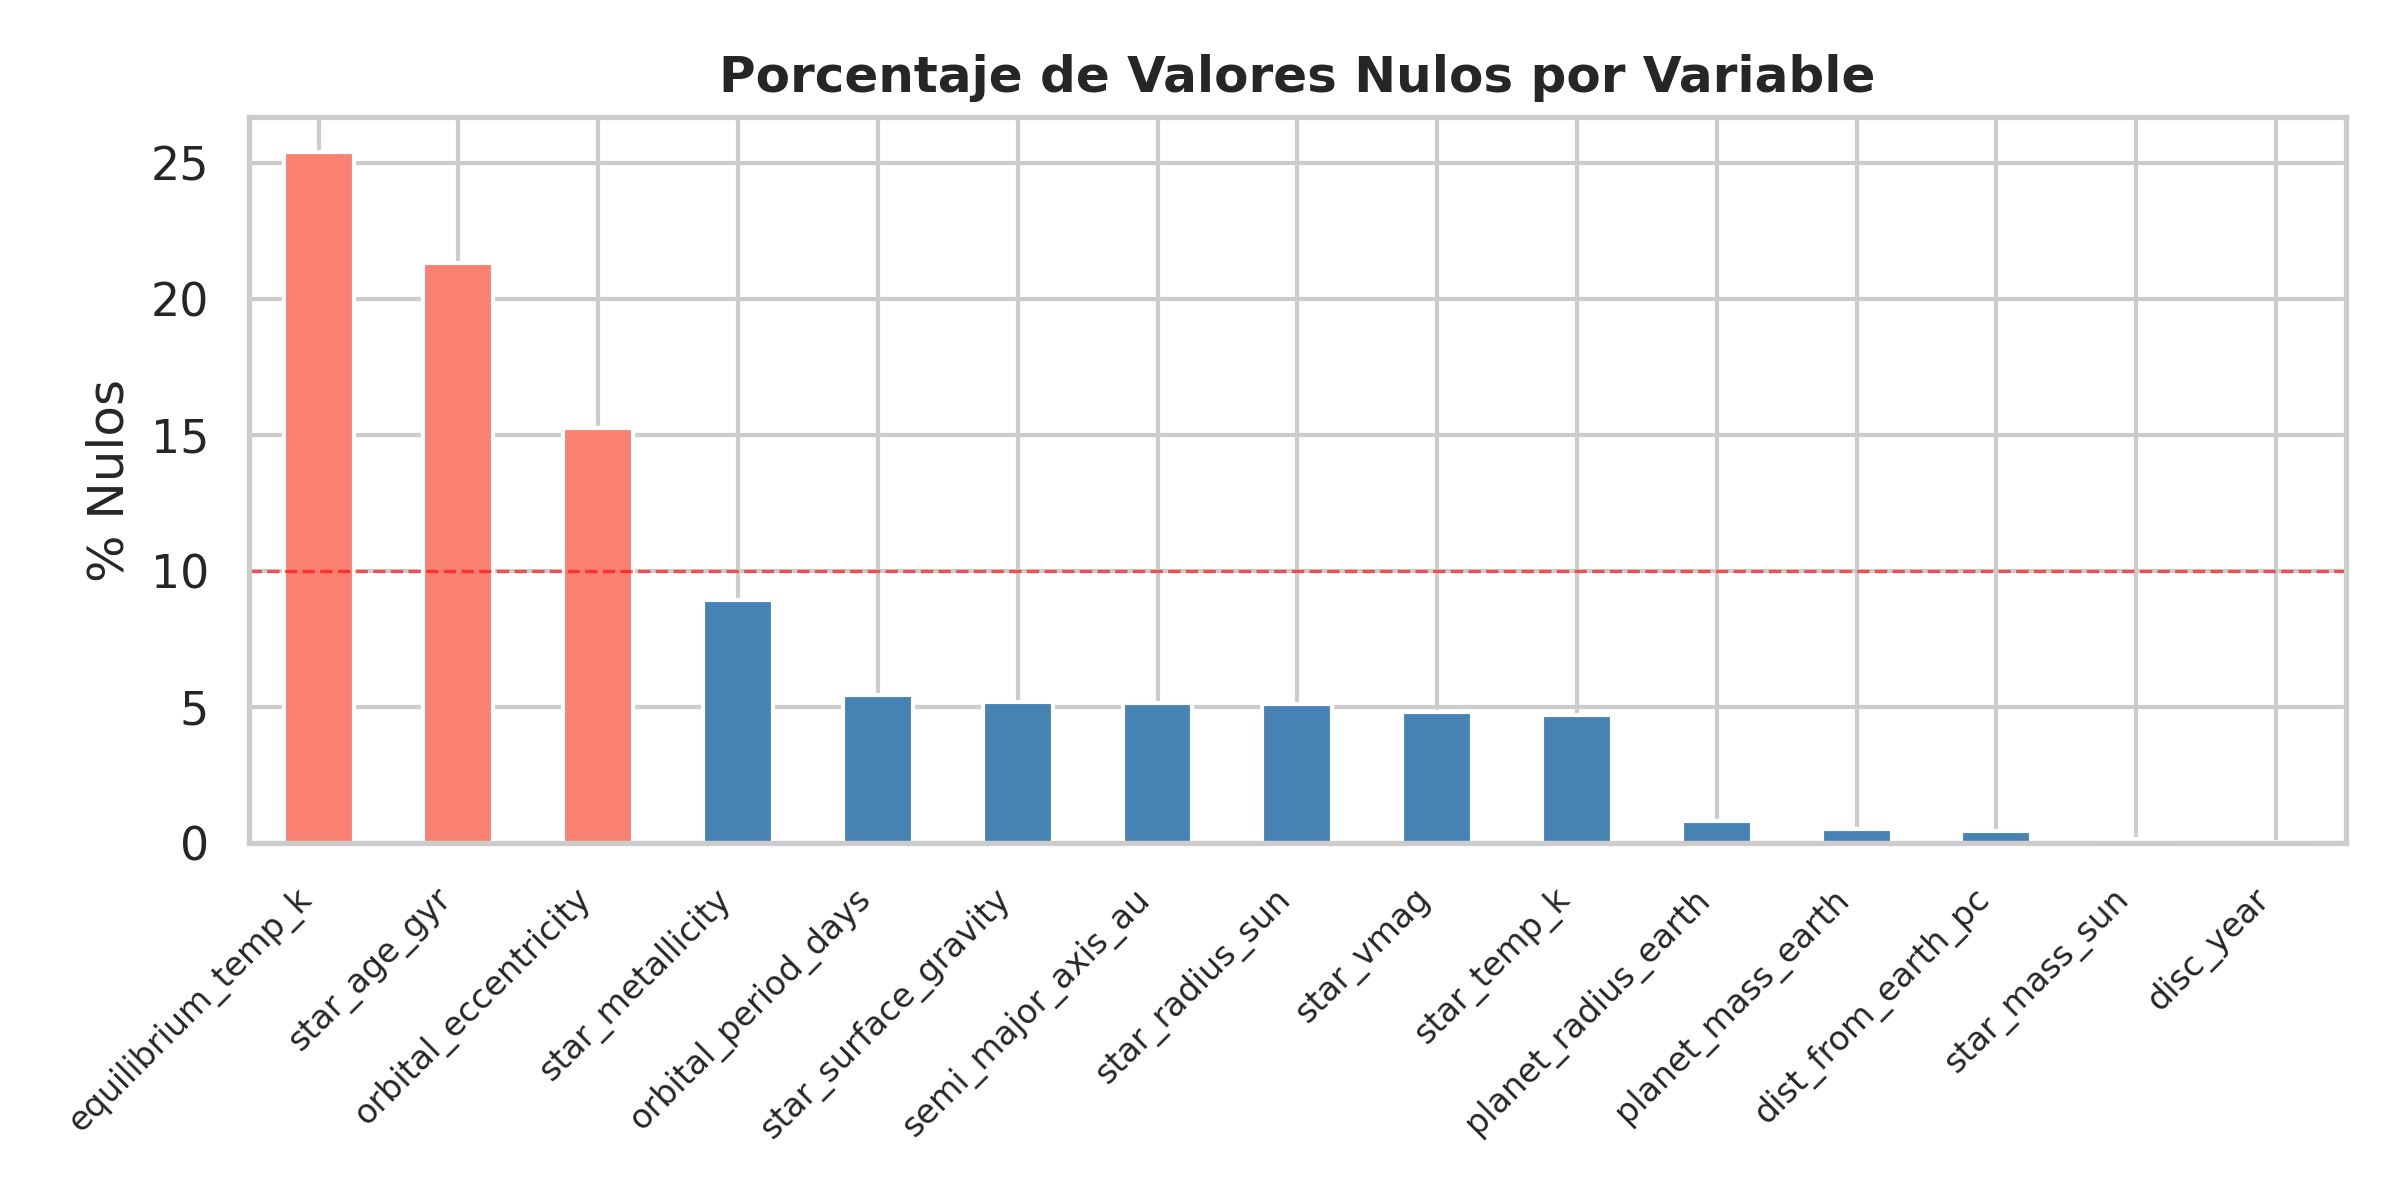
\includegraphics[width=\linewidth]{assets/images/fig_nulos.png}
    \caption{Porcentaje de valores nulos por variable en el conjunto de datos.}
    \label{fig:nulos}
  \end{figure}

  Variables como \texttt{equilibrium\_temp\_k} (25.4\,\%) y \texttt{star\_age\_gyr} (21.3\,\%) fueron descartadas como predictores por su excesiva falta de datos. En cambio, \texttt{orbital\_eccentricity} presenta un 15.25\,\% de nulos, convirti\'endola en una variable objetivo id\'eana para imputaci\'on predictiva.

  La distribuci\'on del target (Figura~\ref{fig:target_dist}) evidencia una marcada asimetr\'ia positiva, con el 75\,\% de los valores por debajo de $e=0.25$, reflejando la predominancia de \'orbitas casi circulares en los descubrimientos actuales.

  \begin{figure}[H]
    \centering
    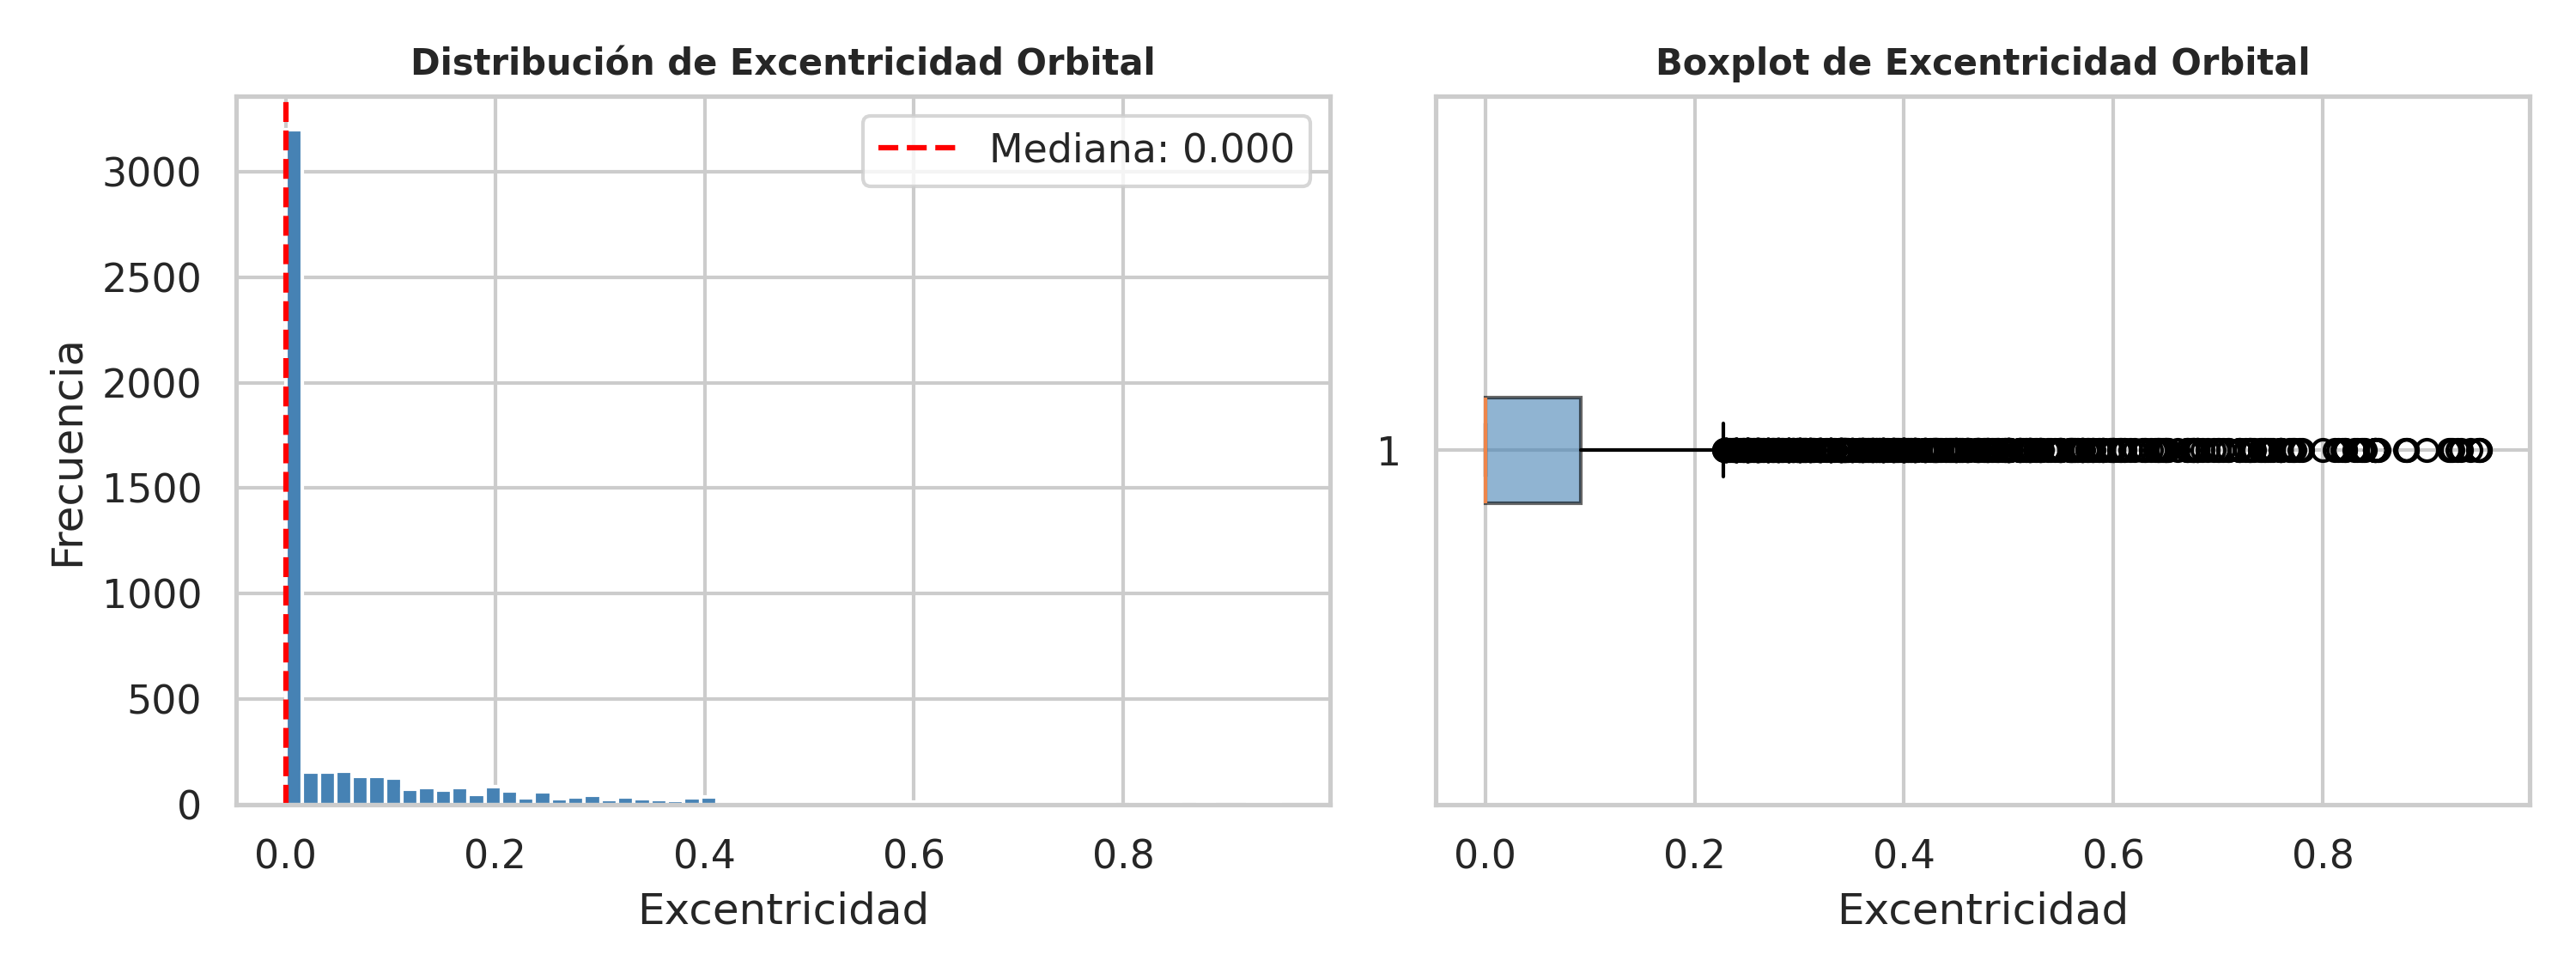
\includegraphics[width=\linewidth]{assets/images/fig_target_dist.png}
    \caption{Histograma y boxplot de la variable objetivo \texttt{orbital\_eccentricity}.}
    \label{fig:target_dist}
  \end{figure}

  \subsection{An\'alisis de Correlaci\'on}

  Se evalu\'o la correlaci\'on de Pearson entre las 13 variables seleccionadas y la excentricidad (Figura~\ref{fig:correlaciones}). Las correlaciones m\'as elevadas corresponden a la magnitud visual estelar \texttt{star\_vmag} ($r = -0.46$), la masa planetaria \texttt{planet\_mass\_earth} ($r = +0.41$) y el radio planetario \texttt{planet\_radius\_earth} ($r = +0.39$).

  \begin{figure}[H]
    \centering
    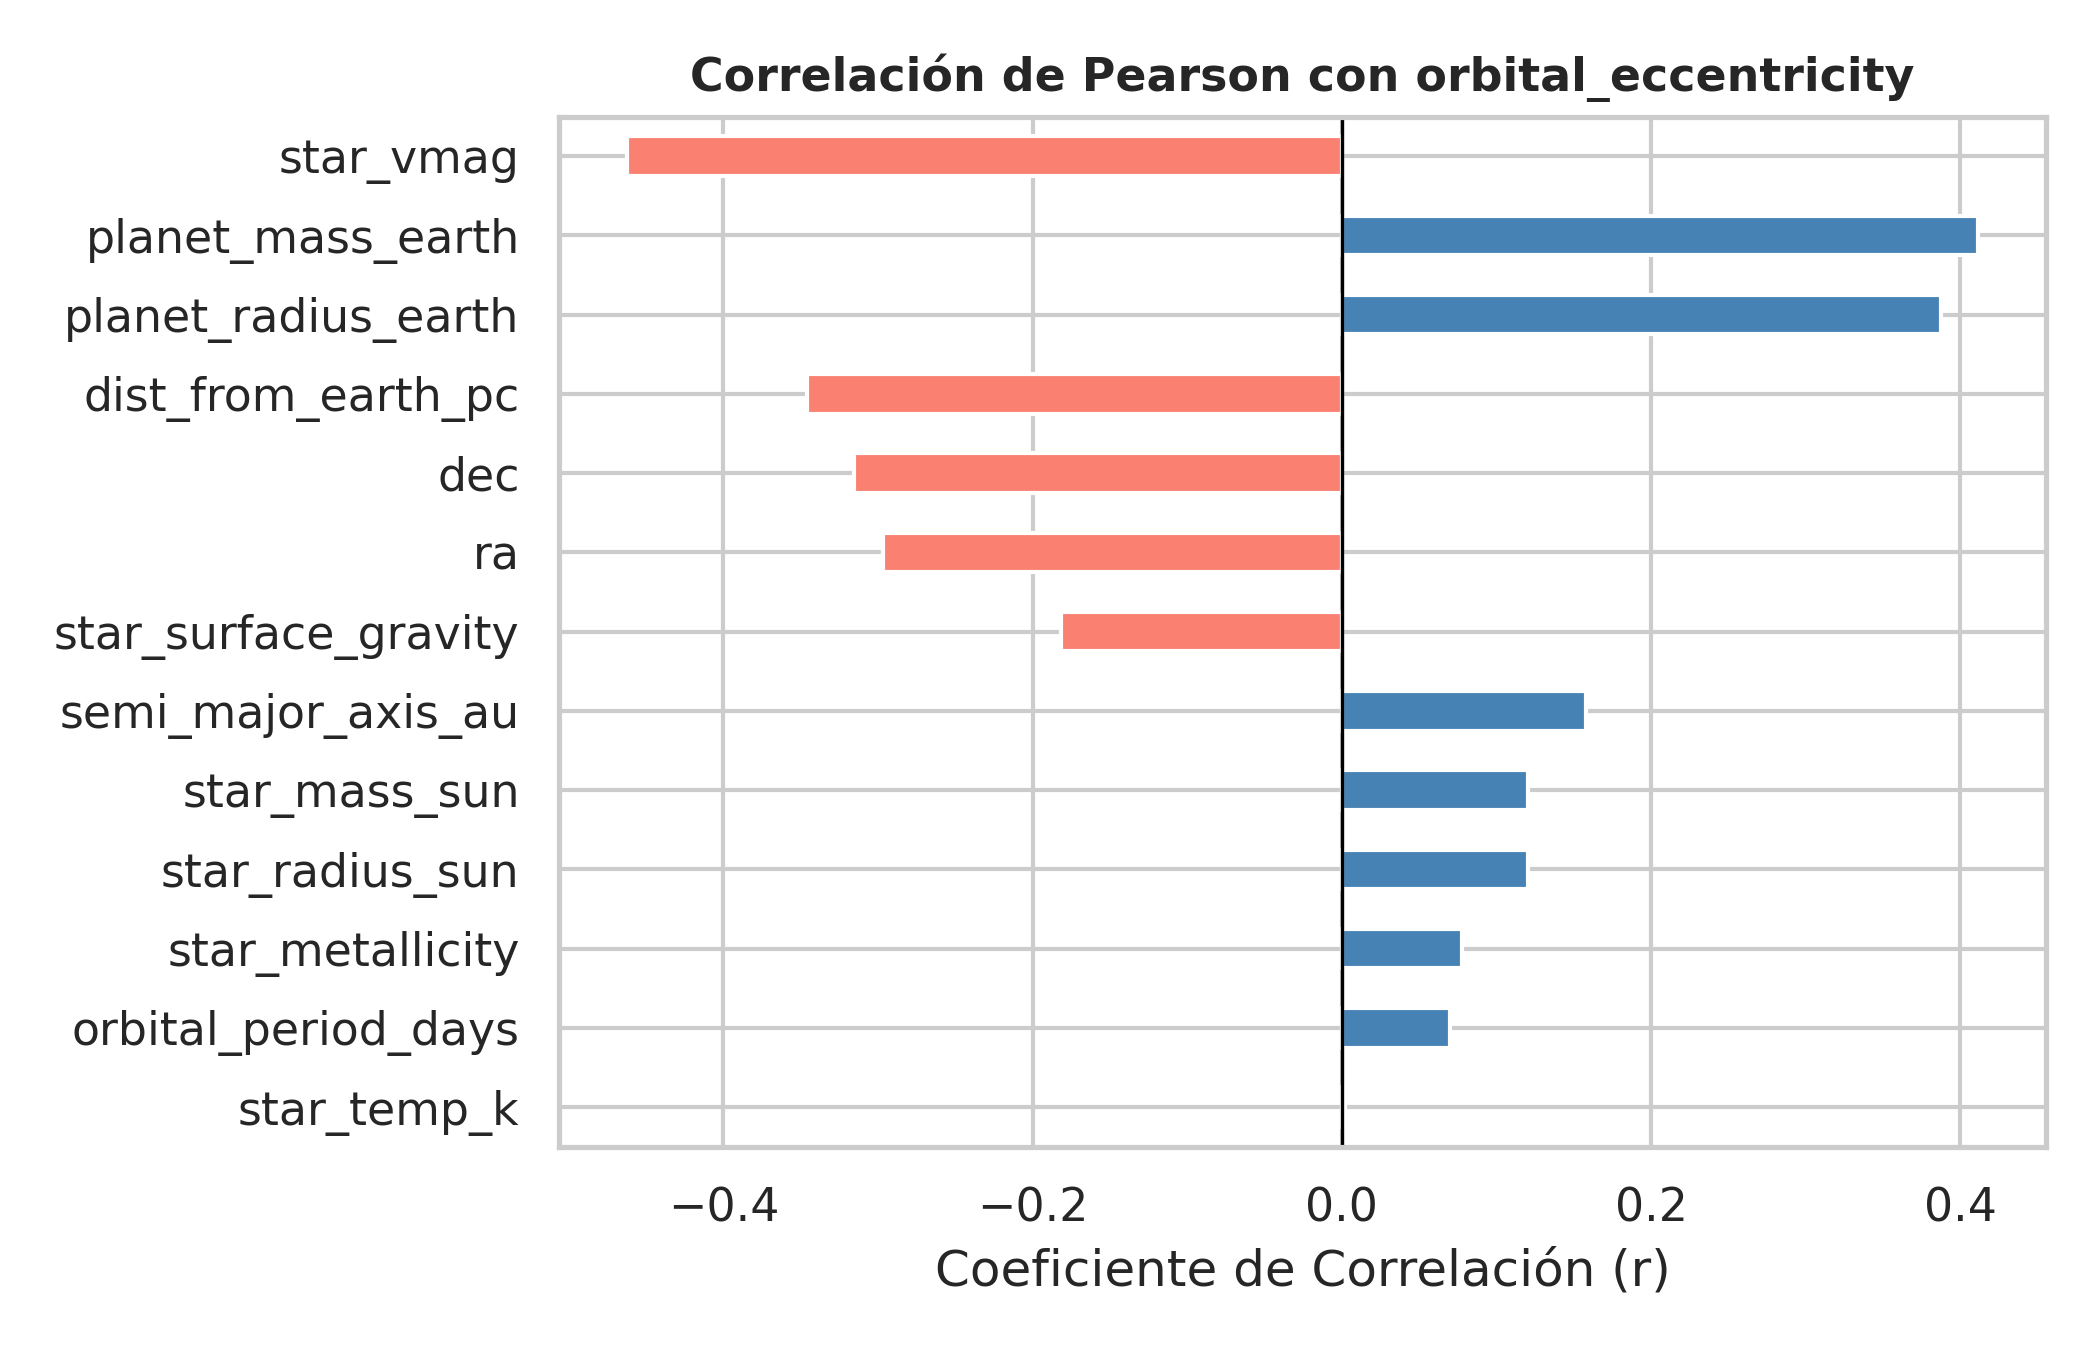
\includegraphics[width=\linewidth]{assets/images/fig_correlaciones.png}
    \caption{Correlaci\'on de Pearson de cada variable predictora con \texttt{orbital\_eccentricity}.}
    \label{fig:correlaciones}
  \end{figure}

  Dado que ning\'un predictor individual supera un $|r| > 0.5$, se concluye que no existe una relaci\'on lineal fuerte directa, lo que fundamenta la necesidad de probar algoritmos no lineales de aprendizaje supervisado.

  \subsection{Preprocesamiento}

  Tras eliminar las filas con nulos en las variables de inter\'es, se obtuvieron 4\,924 registros limpios. La partici\'on de datos se realiz\'o en una proporci\'on 80\,\% para entrenamiento (3\,939 muestras) y 20\,\% para prueba (985 muestras) con \texttt{random\_state=42}.

  Para la Regresi\'on Lineal, se aplic\'o estandarizaci\'on con \texttt{StandardScaler} ($z = \frac{x - \mu}{\sigma}$) sobre los predictores para corregir las diferencias de escala entre magnitudes como el per\'iodo orbital (d\'ias) y la masa.

  \section{Metodolog\'ia de Modelado}

  \subsection{Regresi\'on Lineal (Baseline)}
  Modela el target como $\hat{y} = \beta_0 + \sum_{i=1}^{p} \beta_i x_i$, estimando los coeficientes mediante M\'inimos Cuadrados Ordinarios (OLS) sobre las variables estandarizadas \cite{hastie2009}.

  \subsection{Random Forest}
  Consiste en un ensamble de 100 \'arboles de decisi\'on ($n\_estimators=100$, $min\_samples_leaf=2$) entrenados mediante muestreo bootstrap \cite{breiman2001, amat_rodrigo_2026}. La predicci\'on final corresponde al promedio de las salidas individuales.

  La evaluaci\'on de ambos modelos combin\'o m\'etricas sobre el conjunto de prueba reservado ($R^2$, $RMSE$, $MAE$) y validaci\'on cruzada de 5 pliegues ($k$-fold CV) \cite{pedregosa2011}.

  \section{Resultados y Discusi\'on}

  La Tabla~\ref{tab:resultados} y la Figura~\ref{fig:comparacion} resumen el desempe\~no comparativo de ambos modelos.

  \begin{table}[H]
    \caption{M\'etricas comparativas en conjunto de prueba y validaci\'on cruzada}
    \label{tab:resultados}
    \centering
    \begin{tabular}{lcc}
      \toprule
      \textbf{M\'etrica} & \textbf{Regresi\'on Lineal} & \textbf{Random Forest} \\
      \midrule
      $R^2$ (Test)             & 0.2721 & \textbf{0.3850} \\
      RMSE (Test)              & 0.1158 & \textbf{0.1065} \\
      MAE (Test)               & 0.0681 & \textbf{0.0578} \\
      $R^2$ CV-5fold           & $0.3166 \pm 0.0415$ & $\mathbf{0.4180 \pm 0.0291}$ \\
      \bottomrule
    \end{tabular}
  \end{table}

  \begin{figure}[H]
    \centering
    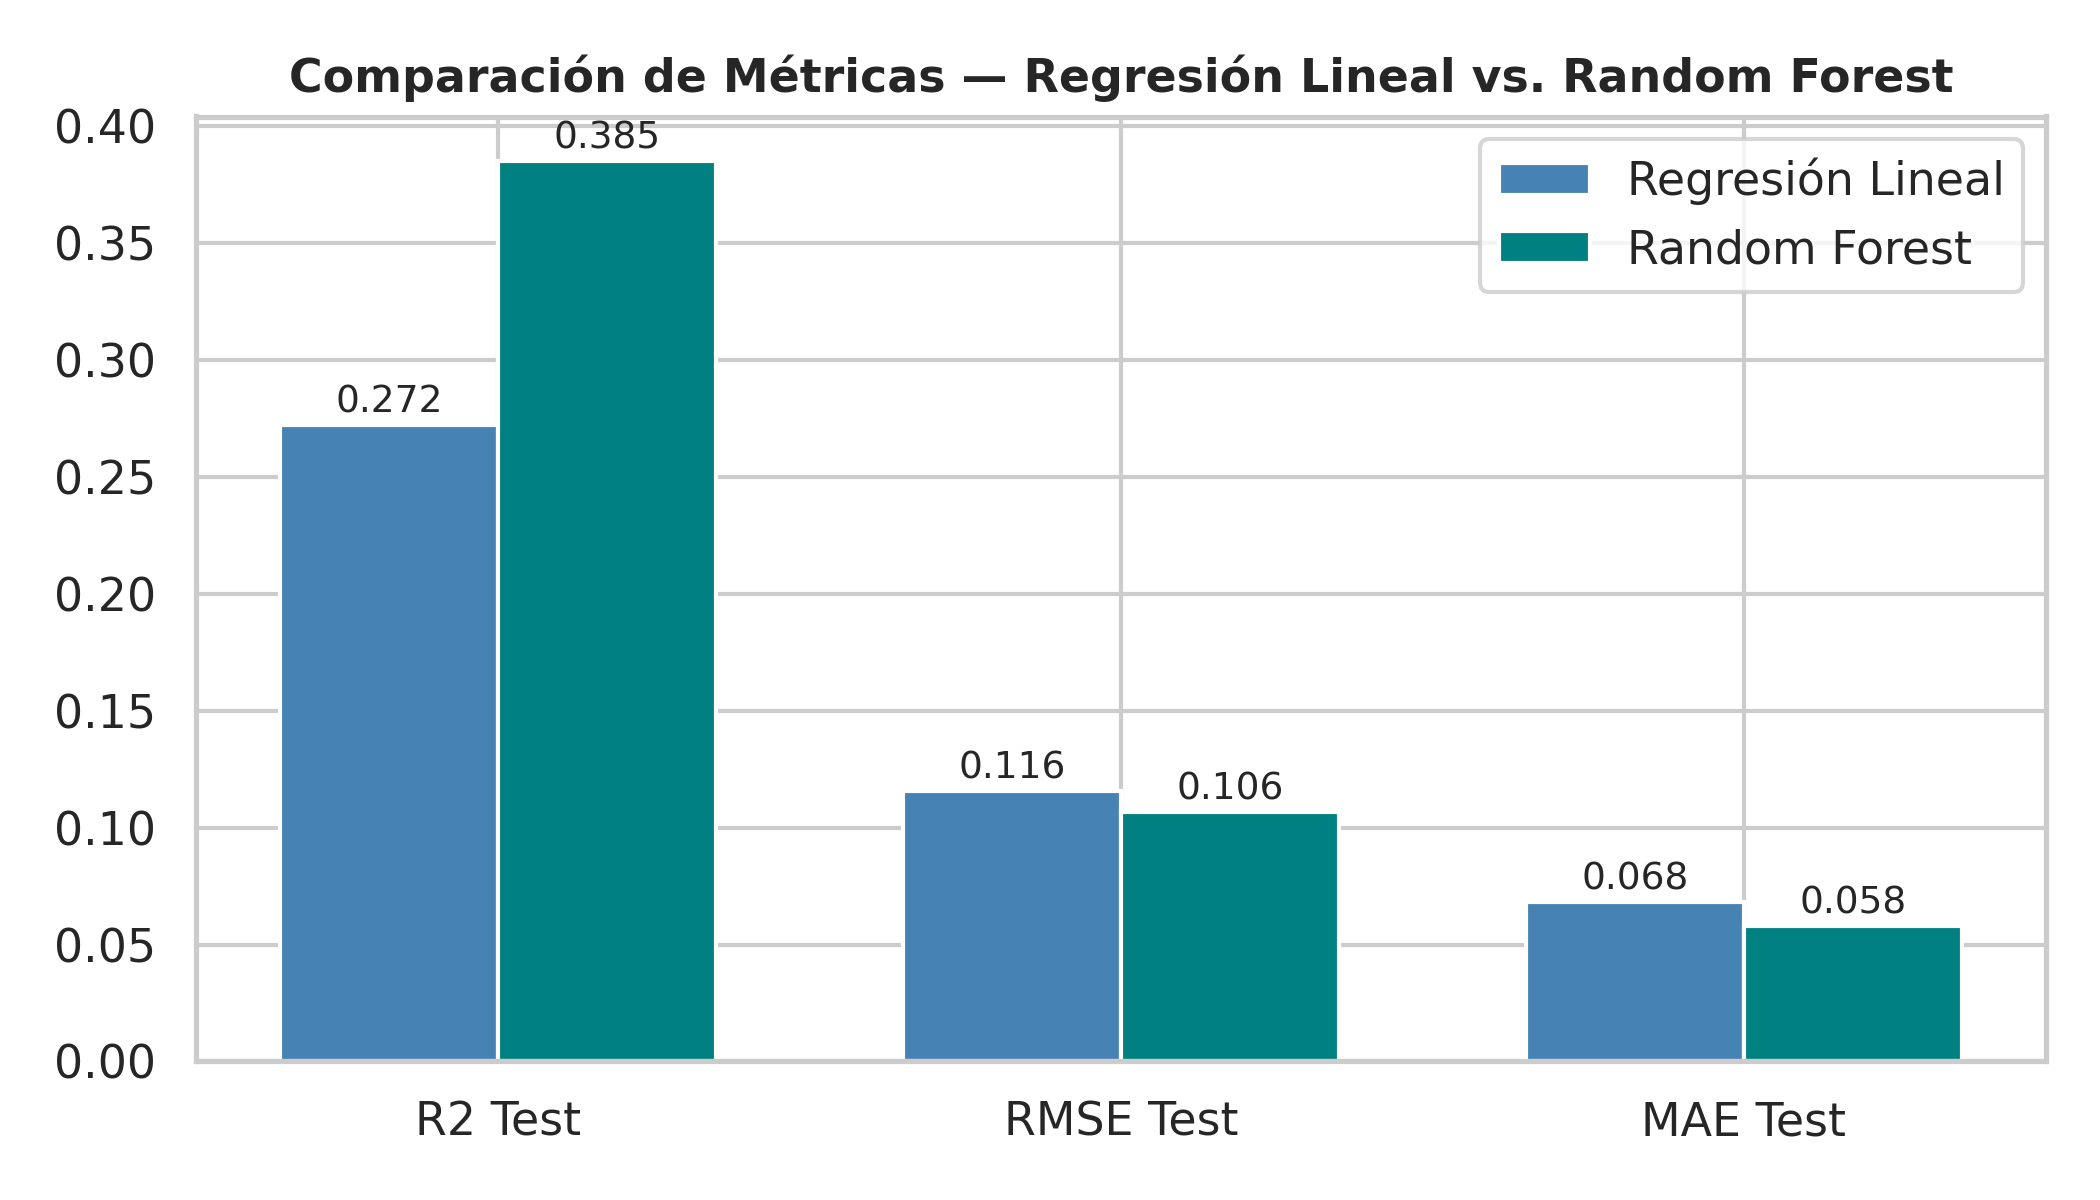
\includegraphics[width=\linewidth]{assets/images/fig_comparacion_modelos.png}
    \caption{Comparaci\'on de m\'etricas $R^2$, $RMSE$ y $MAE$ entre modelos.}
    \label{fig:comparacion}
  \end{figure}

  El modelo \textbf{Random Forest} super\'o a la Regresi\'on Lineal en todas las m\'etricas, alcanzando un $R^2 = 0.3850$ en test y $0.4180$ en validaci\'on cruzada. El an\'alisis de importancia de variables y residuos para Random Forest se presenta en la Figura~\ref{fig:rf_diag}.

  \begin{figure}[H]
    \centering
    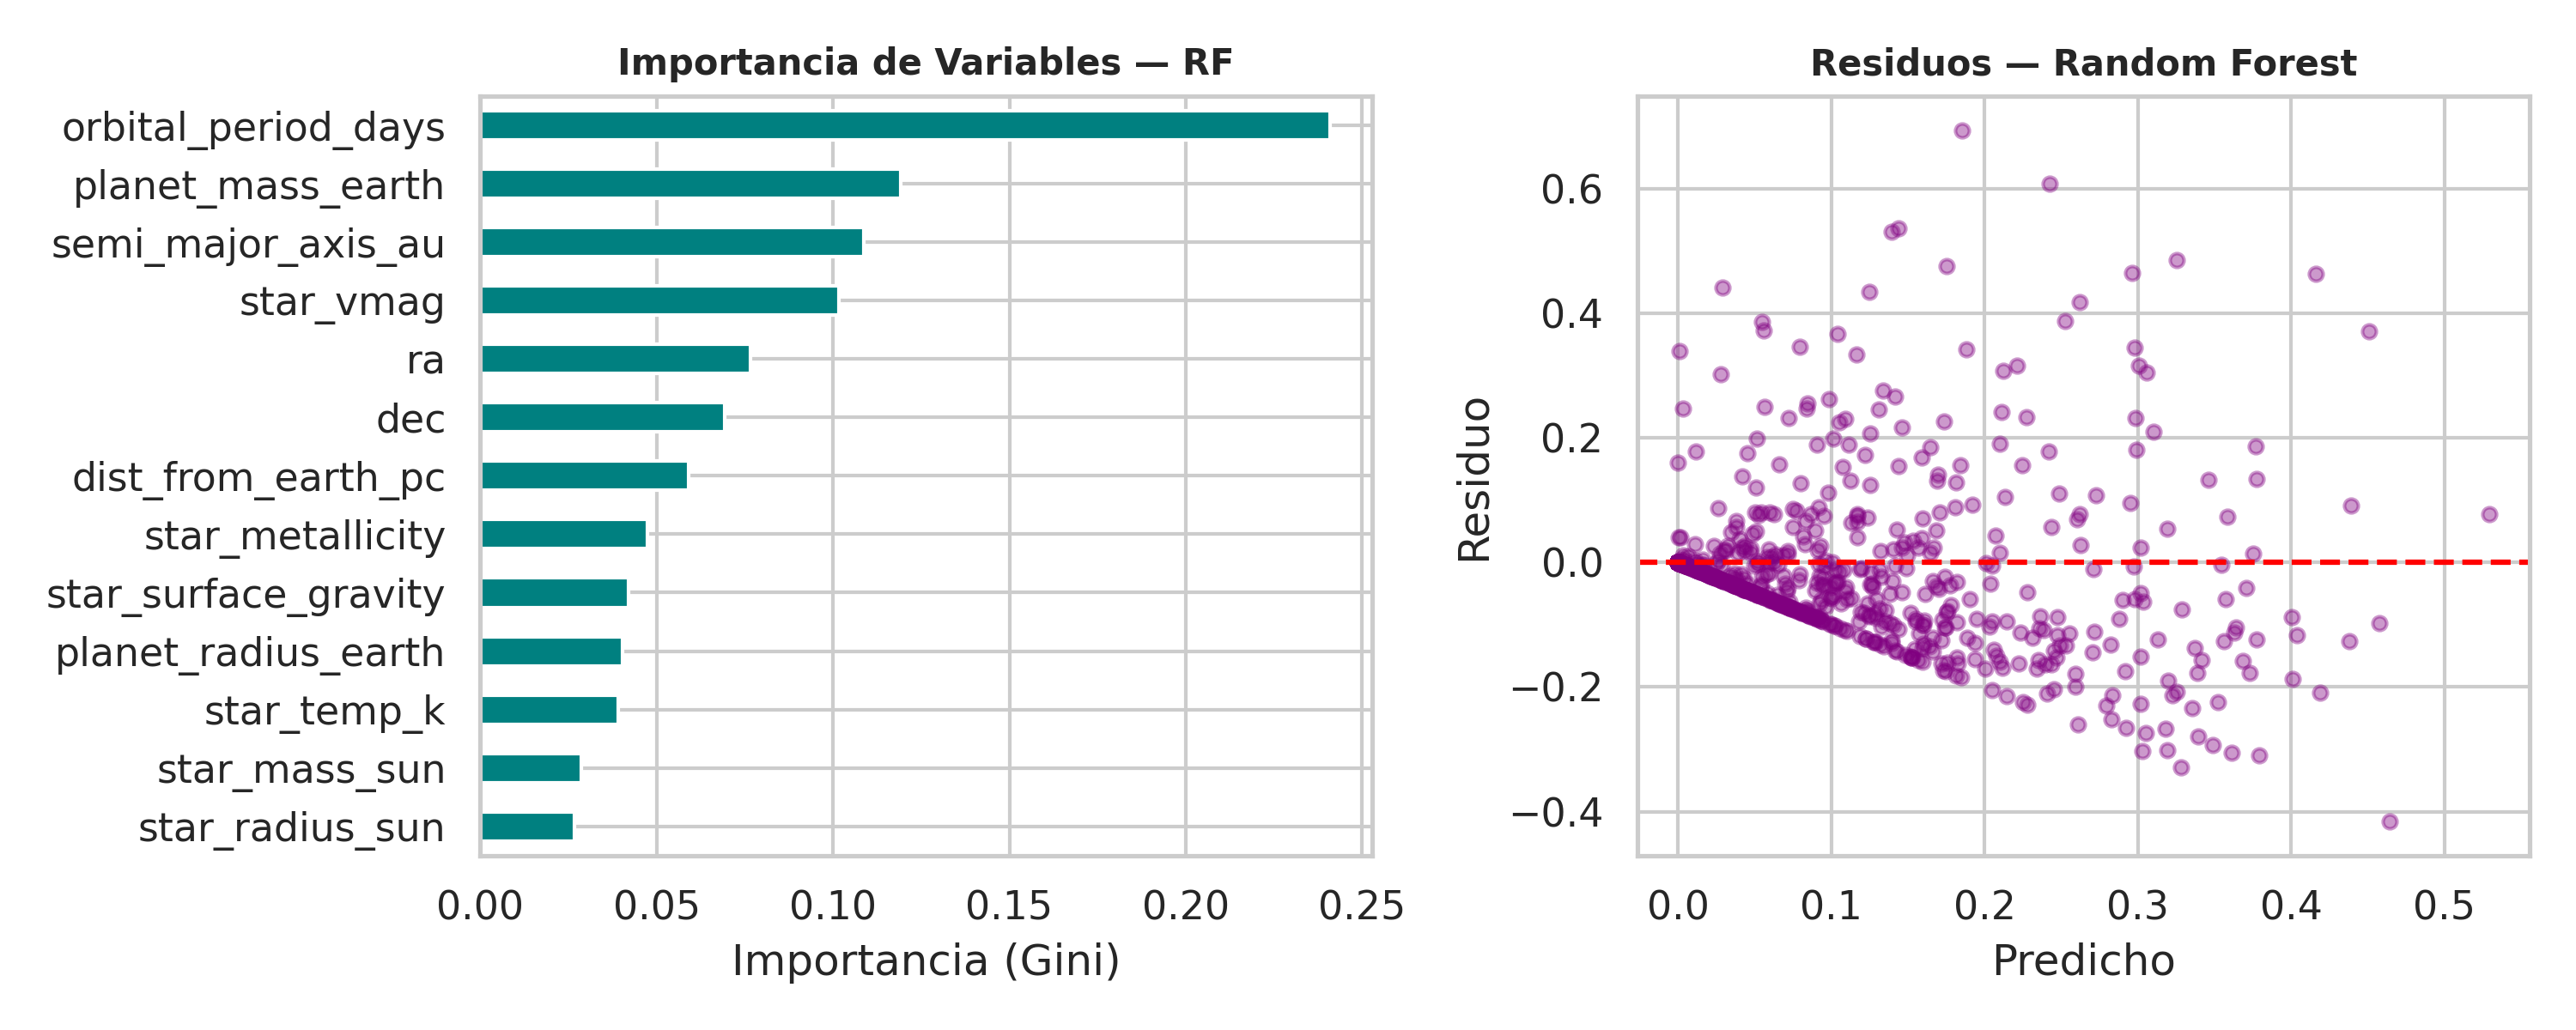
\includegraphics[width=\linewidth]{assets/images/fig_rf_diagnostico.png}
    \caption{Importancia de variables (Gini) y distribuci\'on de residuos para Random Forest.}
    \label{fig:rf_diag}
  \end{figure}

  \section{Conclusiones}

  \begin{enumerate}
    \item \textbf{Random Forest supera a la Regresi\'on Lineal:} El incremento en $R^2$ de 0.2721 a 0.3850 confirma la existencia de patrones no lineales en la excentricidad orbital.
    \item \textbf{Predictores dominantes:} La masa del planeta, el radio planetario y la magnitud estelar son las variables de mayor peso predictivo.
    \item \textbf{Aplicabilidad y Reprodubilidad:} El modelo de ensamble desarrollado en el marco académico de la Universidad de La Salle permite estimar la excentricidad en los exoplanetas con datos faltantes. El experimento completo es totalmente reproducible a trav\'es del cuaderno publicado en Google Colab: \url{https://colab.research.google.com/drive/1UB8g-jYuwyeEerVtnyryVKVM9uYLOb07?usp=sharing}.
  \end{enumerate}

  \bibliographystyle{IEEEtran}
  \bibliography{bib/references}

\end{document}
